% Raport z bloku 3 (codebook, gold standard, walidacja instrumentów) i z testu hipotez.
% Tabele i wykresy generuje `make report-tables` (scripts/13_report_tables.py) z plików wyników,
% więc liczby w tabelach nie są przepisywane ręcznie. Liczby w tekście trzeba sprawdzać z tabelami
% po każdym ponownym przeliczeniu. Kompilacja: pdflatex raport.tex (dwa razy) albo Overleaf
% z całym katalogiem report/.
\documentclass[11pt,a4paper]{article}

\usepackage[utf8]{inputenc}
\usepackage[T1]{fontenc}
\usepackage[polish]{babel}
\usepackage{lmodern}
\usepackage{microtype}
\usepackage[margin=2.3cm]{geometry}
\usepackage{booktabs}
\usepackage{graphicx}
\usepackage{caption}
\usepackage{amsmath}
\usepackage[hidelinks]{hyperref}

\captionsetup{font=small,labelfont=bf}
\graphicspath{{figures/}}
\newcommand{\kod}[1]{\texttt{#1}}
\newcommand{\tabela}[1]{{\small\input{tables/#1}}}
\newcommand{\szeroka}[1]{\resizebox{\linewidth}{!}{\input{tables/#1}}}
\newcommand{\uwaga}[1]{\par\smallskip{\footnotesize #1\par}}

\title{Powoływanie się na źródła w dyskusjach online:\\codebook, gold standard i walidacja instrumentów AI\\
\large Reddit 2005--2020 i Wikipedia 2020--2026}
% Autorzy według historii repozytorium; dopisać pozostałe osoby zespołu, jeśli są.
\author{Jan Poręba \and Igor Sosnowicz}
\date{Analiza Mediów Cyfrowych, projekt \kod{digital-media-analysis}\\25 października 2026}

\begin{document}
\maketitle

\begin{abstract}
Badamy, jak użytkownicy Reddita (lata 2005--2020) i redaktorzy polskiej Wikipedii (lata 2020--2026) powołują się na źródła informacji. Zbudowaliśmy codebook z dziewięcioma kategoriami źródeł, losową próbę warstwową 500 jednostek na platformę z wagami do ramy losowania i etykiety referencyjne (gold standard). Na tych etykietach porównaliśmy pięć instrumentów: zamrożone reguły z analizy eksploracyjnej (v1), model zero-shot NLI, ekstraktor wzmianek GLiNER, reguły v2 napisane według codebooka i miarę zmiany przypisów w treści artykułu (I4). Na Reddicie GLiNER wykrywa powołania prawie bezbłędnie (F1 0,96 na zbiorze testowym), ale typ źródła rozpoznaje tylko umiarkowanie (MASI 0,46). Na Wikipedii żaden z przetestowanych instrumentów nie mierzy typów źródeł wiarygodnie: to wynik negatywny. Zgodność annotatorów w pilotażu była niska, a wyniki instrumentów zależą od tego, czyje etykiety są punktem odniesienia. Hipoteza H1 (spadek zaufania do konsensusu naukowego) nie ma jeszcze testu głównego; wskaźniki źródeł jej nie wspierają, bo zmiany w danych łącznych wynikają ze zmiany składu subredditów. Hipoteza H2 (więcej źródeł alternatywnych) formalnie przeszła test z preregistracji, ale sprawdzenie pomiaru pokazało, że wynik jest artefaktem klasyfikacji linków po domenie.
\end{abstract}

\section{Wprowadzenie}

Projekt odpowiada na dwa pytania badawcze, zapisane jako hipotezy przed analizą potwierdzającą (preregistracja w \kod{docs/hipotezy.md}):
\begin{itemize}
  \item \textbf{H1:} w latach 2005--2018 w przestrzeni online maleje zaufanie do konsensusu naukowego (Reddit);
  \item \textbf{H2:} w latach 2020--2026 użytkownicy częściej odwołują się do alternatywnych źródeł wiedzy, takich jak blogi, influencerzy i „eksperci niezależni” (Wikipedia).
\end{itemize}
Obie hipotezy wymagają zmierzenia, na jakie źródła powołują się autorzy, na dziesiątkach tysięcy jednostek. Ręcznie się tego nie zrobi, więc kluczowe jest pytanie metodologiczne: czy instrument automatyczny mierzy to, co opisuje codebook, i z jakim błędem? Raport opisuje kolejno codebook (sekcja~\ref{sec:codebook}), gold standard (sekcja~\ref{sec:gold}), instrumenty i ich walidację (sekcje~\ref{sec:instrumenty}--\ref{sec:porownanie}), a na końcu hipotezy (sekcja~\ref{sec:hipotezy}).

\section{Dane i próba}
\label{sec:dane}

Wszystkie skrypty pobierają i losują tylko źródła wymienione w pliku konfiguracyjnym \kod{config.yaml}:
\begin{itemize}
  \item \textbf{Reddit:} sześć polskich subredditów oraz r/reddit.com (tylko 2005~r.), r/science (od 2006~r.), r/skeptic i r/conspiracy (od 2008~r.).
  \item \textbf{Wikipedia:} osiem polskich artykułów o zdrowiu i klimacie.
\end{itemize}

Ramą Reddita są wszystkie posty z jednego losowego dnia każdego miesiąca, dla każdego subredditu i roku. Subreddit z mniej niż 100 postami w wylosowanych dniach wchodzi za dany rok w całości. Rama liczy 62\,636 widocznych postów; posty usunięte nie wchodzą do ramy. Ramą Wikipedii jest 1453 rewizji z niepustym opisem zmiany. Jednostką analizy jest post (tytuł, treść i link) albo opis zmiany.

Próba gold liczy 500 jednostek na platformę. Jest rozłożona między lata tak równo, jak pozwalają dane, więc oszacowania roczne mają podobną precyzję. Warstwą jest rok, a na Wikipedii rok $\times$ sygnał powierzchniowy (link, słowa o źródłach, reszta). Waga jednostki to $N_h/n_h$, czyli liczba jednostek warstwy w ramie przez liczbę jednostek zakodowanych w tej warstwie. Na Reddicie waga uwzględnia też wylosowany dzień.

Próba dzieli się na:
\begin{itemize}
  \item pilotaż, który nie wchodzi do ramy próby głównej;
  \item zbiór \kod{dev} do strojenia instrumentów;
  \item zbiór \kod{test}, uruchamiany dla każdego instrumentu raz, po zamrożeniu kodu commitem.
\end{itemize}
Drugą rundę pilotażu (\kod{pilot2}) wylosowano spoza próby, żeby nie naruszać zbioru testowego. Tabela~\ref{tab:proba} podaje liczności.

\begin{table}[htbp]
\centering
\caption{Liczności próby gold według fazy i podziału oraz jednostki zakodowane w gold (podział między osoby IS i JP).}
\label{tab:proba}
\tabela{sample}
\uwaga{Gold jest podzielony między dwie osoby: każda jednostka ma jedną etykietę. Zgodność mierzymy na pilotażu, który kodowały obie osoby.}
\end{table}

\section{Codebook}
\label{sec:codebook}

\textbf{Konstrukt i zmienne.} Konstruktem jest powołanie się na źródło informacji: tekst lub link wskazuje, skąd pochodzi informacja, albo podaje ją jako podstawę twierdzenia. Codebook v2.1 (\kod{codebook/codebook.yaml}, instrukcja \kod{codebook.md}) zastąpił dwa niezgodne schematy kategorii z analizy eksploracyjnej jednym schematem dla obu platform. Ma cztery zmienne:
\begin{itemize}
  \item \kod{source\_types}: zbiór kategorii z tabeli~\ref{tab:kategorie}; \kod{none} oznacza brak powołania;
  \item \kod{cites\_source}: wyliczana z \kod{source\_types} (0 przy \kod{none});
  \item \kod{edit\_about\_sources}: tylko Wikipedia, deklaracja pracy nad przypisami w opisie zmiany;
  \item \kod{consensus\_stance}: tylko Reddit, stanowisko wobec konsensusu naukowego (dla H1-A).
\end{itemize}

\begin{table}[htbp]
\centering
\caption{Kategorie zmiennej \kod{source\_types} (codebook v2.1).}
\label{tab:kategorie}
\tabela{categories}
\end{table}

\textbf{Reguły rozstrzygania.} Kluczowe reguły odpowiadają na błędy, które wyszły w analizie eksploracyjnej:
\begin{itemize}
  \item R2: powołanie wymaga funkcji źródła, więc instytucja jako temat posta się nie liczy;
  \item R3: własne zdjęcia z i.redd.it czy imgur, ankiety i reklamy nie są źródłem;
  \item R4: kategorię wyznacza wydawca, a nie temat;
  \item R5: konkretne źródło wygrywa z ogólnikiem;
  \item R8: opinia ani prośba o źródło nie są powołaniem;
  \item R9: skróty \kod{[[WP:...]]}, prefiks sekcji i rewerty są elementami technicznymi Wikipedii;
  \item R10: znacznik „źródła/przypisy” daje \kod{edit\_about\_sources} = 1, a nie kategorię źródła.
\end{itemize}

Instrument v1 łamał te reguły na dużą skalę. Wśród jego wzmianek w Wikipedii 274 z 485 to skróty \kod{WP:}, a 88 to znaczniki typu edycji. Na Reddicie v1 nie widział linku posta w 124 z 275 postów, bo czytał tylko treść.

\section{Gold standard}
\label{sec:gold}

\subsection{Proces annotacji i zgodność}

Annotatorzy kodowali w arkuszach bez wyników żadnego instrumentu, według codebooka i instrukcji krok po kroku osobnych dla każdej platformy. Pilotaż (32 posty i 20 opisów zakodowanych przez obie osoby) dał niską zgodność (tabela~\ref{tab:pilot}, rysunek~\ref{fig:pilot}):
\begin{itemize}
  \item \textbf{Reddit, \kod{cites\_source}:} IS uznał za powołujące się na źródło wszystkie 32 posty, a JP 29. Przy 91\% zgodności $\alpha$ Krippendorffa wynosi więc około zera. To paradoks rozpowszechnienia: przy cesze prawie zawsze obecnej miary poprawione o zgodność przypadkową są bliskie zera nawet przy dużej zgodności surowej \cite{feinstein1990}.
  \item \textbf{Reddit, typy źródeł:} $\alpha$ z odległością MASI \cite{passonneau2006} wynosi 0,34, poniżej progu 0,667 \cite{krippendorff2004}.
  \item \textbf{Wikipedia:} powołań było za mało do oceny; \kod{edit\_about\_sources} osiąga $\alpha = 0{,}70$ przy szerokim przedziale.
\end{itemize}
Według reguły zapisanej przed pilotażem potrzebna jest druga runda (\kod{pilot2}, 30 postów i 30 opisów). JP ją zakodował, IS jeszcze nie. Spory z pierwszej rundy (20 jednostek) czekają na arbitra. Arkusz arbitra pokazuje etykiety i notatki obu osób, a decyzje zastępują w gold etykiety sporne.

\begin{table}[htbp]
\centering
\caption{Zgodność annotatorów w pilotażu (pierwsza runda), $\alpha$ Krippendorffa z 95\% przedziałem bootstrap.}
\label{tab:pilot}
\tabela{pilot_agreement}
\uwaga{Zmiennych, które obie osoby razem zaznaczyły w mniej niż 5 jednostkach, nie oceniamy („za mało przypadków”).}
\end{table}

\begin{figure}[htbp]
\centering
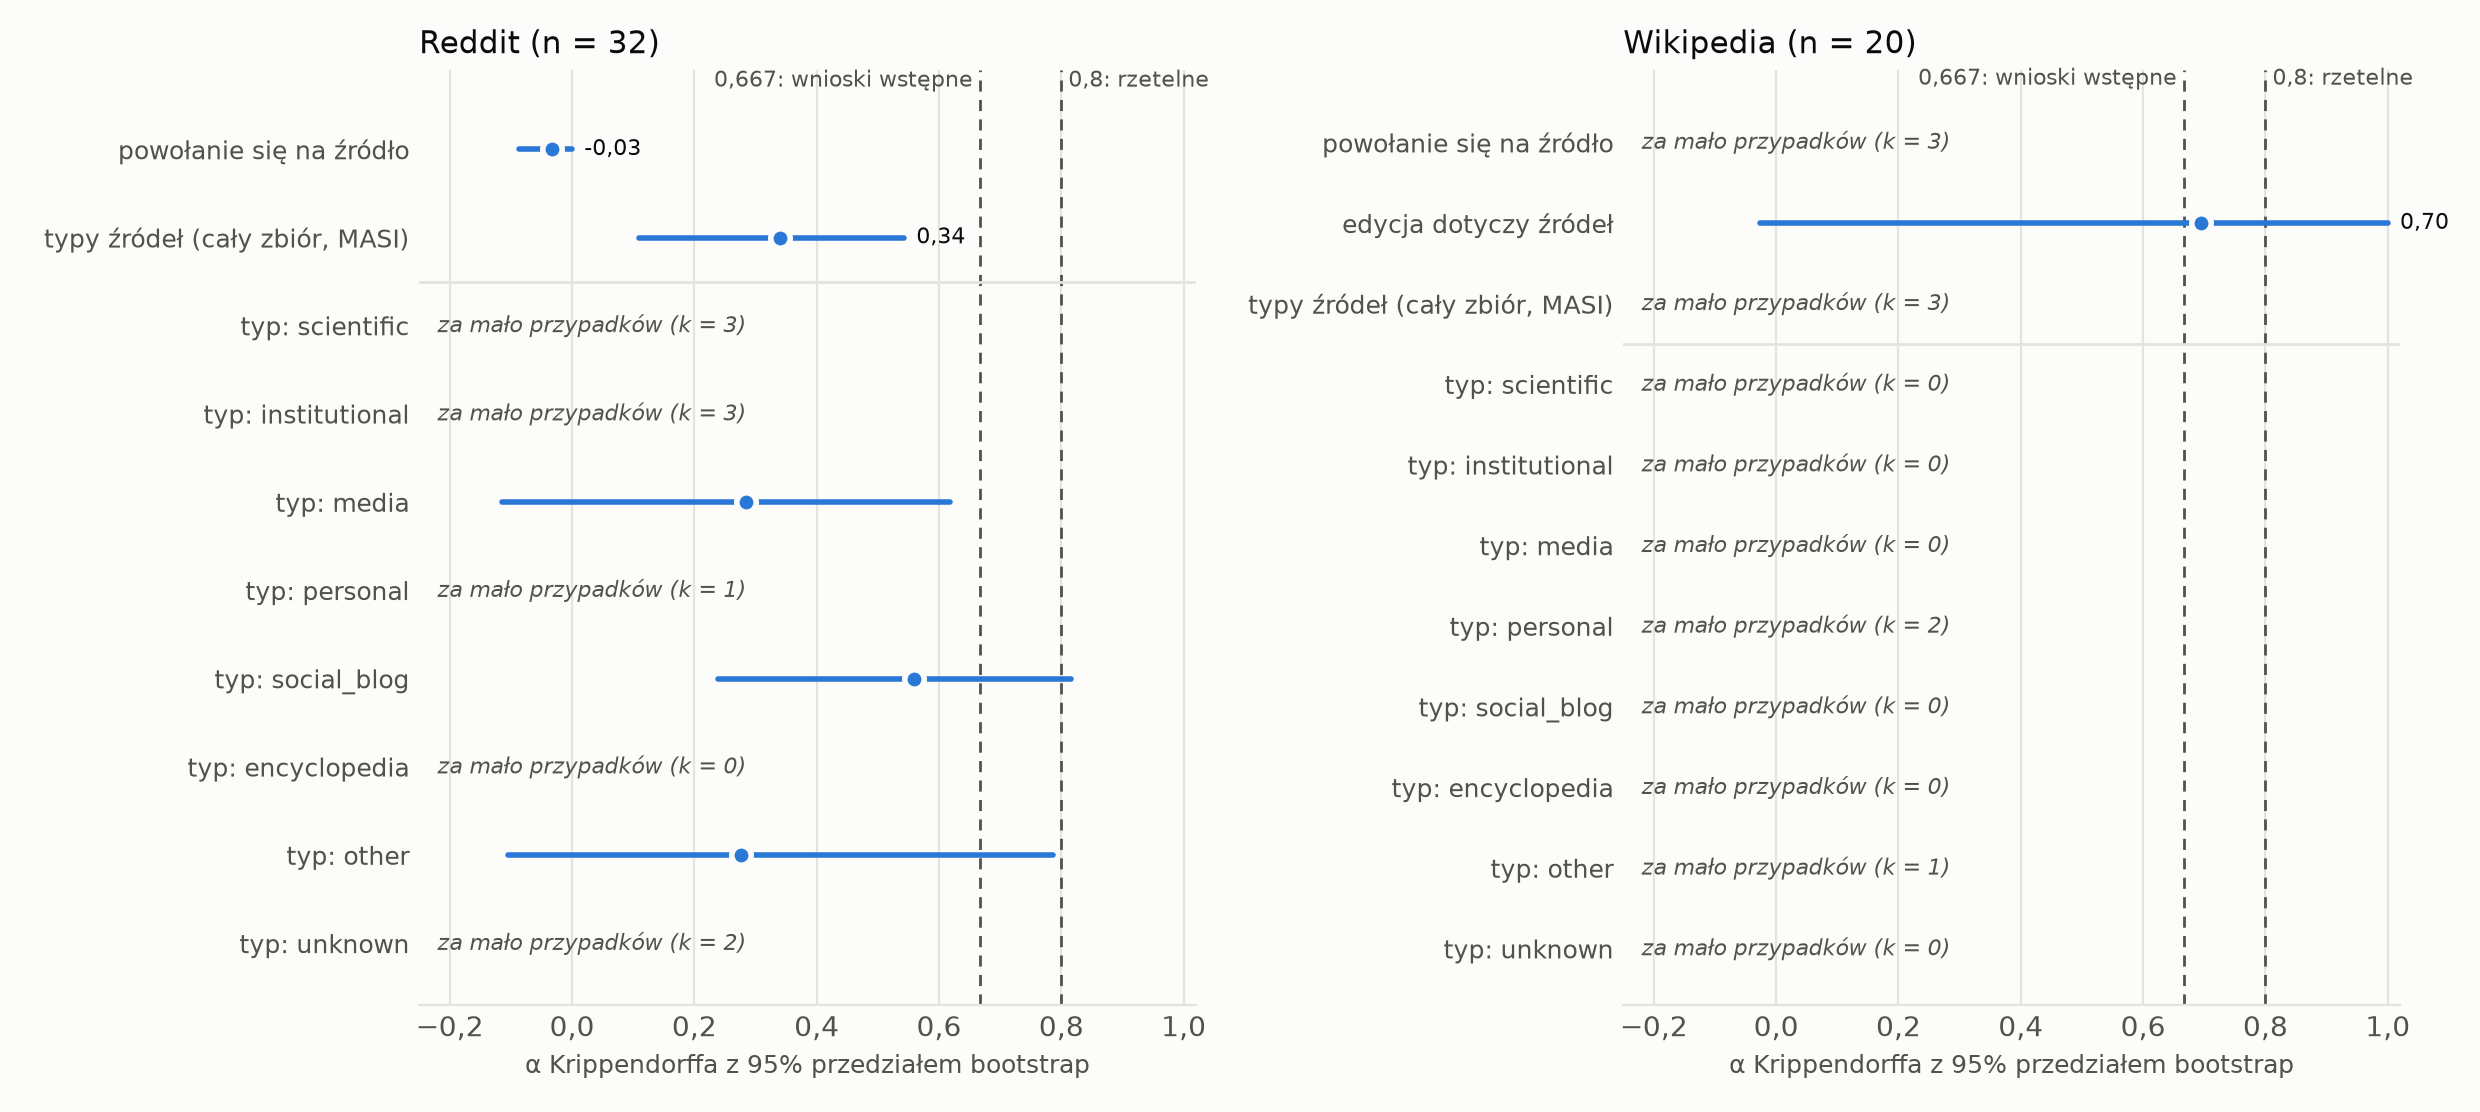
\includegraphics[width=\linewidth]{pilot_alpha.png}
\caption{$\alpha$ Krippendorffa w pilotażu dla zmiennych i kategorii, z progami 0,667 i 0,8.}
\label{fig:pilot}
\end{figure}

\textbf{Etykiety JP i AI.} Etykiety JP w pilotażu i gold powstały z etykiet wstępnych przygotowanych przez asystenta AI według codebooka, bez wglądu w etykiety IS. JP przejrzał wszystkie wiersze i zatwierdził etykiety. Zgodność IS--JP jest więc zgodnością IS z etykietami wspomaganymi przez AI. Ma to też znaczenie przy ocenie instrumentów AI, bo część gold może być im bliższa z powodu wspólnego pochodzenia (sekcja~\ref{sec:walidacja}).

\subsection{Udziały źródeł z samego gold}

Etykiety gold dają estymatę udziałów, która nie zależy od żadnego instrumentu (tabela~\ref{tab:udzialy}):
\begin{itemize}
  \item \textbf{Reddit:} powołanie ma 88\% postów, głównie na media informacyjne (41\%) oraz media społecznościowe i blogi (33\%);
  \item \textbf{Wikipedia:} powołanie zawiera tylko 13\% opisów zmian, a każda kategoria ma najwyżej kilka procent.
\end{itemize}
Etykiety IS i JP różnią się systematycznie, więc estymata dziedziczy ten rozrzut.

\begin{table}[htbp]
\centering
\caption{Ważone udziały jednostek z powołaniem i z każdą kategorią źródła, z etykiet gold (\kod{dev} i \kod{test} razem), z 95\% przedziałami bootstrap w warstwach.}
\label{tab:udzialy}
\tabela{gold_shares}
\end{table}

\section{Instrumenty}
\label{sec:instrumenty}

Wszystkie instrumenty czytają jednostkę tak, jak definiuje ją codebook: na Reddicie tytuł, treść i link (bez własnych mediów autora, R3), na Wikipedii opis zmiany bez prefiksu sekcji (R9). Wynikiem są etykiety w kodach codebooka:
\begin{description}
  \item[v1] Zamrożony ekstraktor słów kluczowych i wyrażeń regularnych z analizy eksploracyjnej, punkt odniesienia. Na Reddicie czyta tylko treść posta i nie mierzy \kod{edit\_about\_sources}.
  \item[zero-shot] Wielojęzyczny model NLI mDeBERTa-v3 \cite{laurer2024} z jedną hipotezą na kategorię; wynik to prawdopodobieństwo wynikania z trzech klas. Strojone na \kod{dev} są próg i język hipotez.
  \item[GLiNER] Wydobywanie wzmianek o źródłach (redakcje, czasopisma, instytucje, serwisy) modelem GLiNER \cite{zaratiana2024}, mapowanych na kategorie. Link bez rozpoznanego typu to \kod{other} (R7).
  \item[reguły v2] Reguły z codebooka zbudowane wyłącznie na \kod{dev}:
    \begin{itemize}
      \item dopasowanie całych słów;
      \item domena linku według słownika domen (R4), a nieznana domena to \kod{other};
      \item bez skrótów \kod{WP:} i rewertów (R9);
      \item znacznik „źródła/przypisy” tylko jako \kod{edit\_about\_sources} (R10);
      \item kategoria z nazwy tuż po sygnale powołania („wg”, „na podstawie”, „according to”), a sam sygnał to \kod{unknown} (R5).
    \end{itemize}
  \item[I4] Tylko Wikipedia, tylko \kod{edit\_about\_sources}: 1, gdy rewizja dodała lub usunęła choć jeden przypis (treść \kod{<ref>} albo szablon \kod{\{\{Cytuj\}\}}) względem poprzedniej rewizji strony.
\end{description}
Modele działają lokalnie, są przypięte do konkretnych commitów z Hugging Face i są deterministyczne, więc żaden tekst nie opuszcza komputera.

\section{Walidacja na gold}
\label{sec:walidacja}

\textbf{Miary.} Instrumenty porównujemy z etykietami gold za pomocą miar ważonych wagami próby, z 95\% przedziałami bootstrap w warstwach:
\begin{itemize}
  \item dla \kod{cites\_source} i \kod{edit\_about\_sources}: precyzja, czułość, F1 i $\kappa$ Cohena \cite{cohen1960};
  \item dla każdej kategorii: F1 (jedna przeciw reszcie), oceniane tylko przy co najmniej 10 przypadkach w gold;
  \item dla całego zbioru typów: średnie podobieństwo MASI i macro-F1.
\end{itemize}
Zbiór testowy uruchomiliśmy raz, na instrumentach zamrożonych commitem \kod{33ff729} (tabela~\ref{tab:test}). Reguły v2 i I4 oceniliśmy na razie tylko na \kod{dev} (tabela~\ref{tab:dev}), czyli na zbiorze, na którym powstały, więc te wyniki są górną granicą.

\begin{table}[htbp]
\centering
\caption{Wyniki na zbiorze testowym (Reddit 78 postów, w tym 68 z powołaniem; Wikipedia 147 opisów, w tym 20 z powołaniem). Miary ważone z 95\% przedziałami bootstrap.}
\label{tab:test}
\tabela{test_metrics}
\uwaga{macro-F1 obejmuje kategorie z co najmniej 10 przypadkami w gold; na Reddicie to \kod{media} i \kod{social\_blog}, na Wikipedii żadna.}
\end{table}

\begin{table}[htbp]
\centering
\caption{Wyniki na zbiorze \kod{dev} dla wszystkich pięciu instrumentów. Reguły v2 i I4 powstały na tym zbiorze, więc ich wyniki są optymistyczne; na teście jeszcze ich nie uruchomiliśmy.}
\label{tab:dev}
\szeroka{dev_metrics}
\end{table}

\textbf{Reddit.} GLiNER znajduje wszystkie powołania (czułość 1,00 przy precyzji 0,93) i jest stabilny między \kod{dev} a \kod{test}. Typ źródła rozpoznaje umiarkowanie: dobrze media i media społecznościowe (F1 0,66 i 0,70), rzadkie kategorie słabo. $\kappa$ dla \kod{cites\_source} jest umiarkowane mimo F1 0,96 z tego samego powodu co w pilotażu, czyli przez rozpowszechnienie. v1 praktycznie nie działa, bo nie czyta linku posta (442 z 500 postów to linki). Na \kod{dev} reguły v2 osiągają wyższe MASI niż GLiNER (0,60 wobec 0,50), bo domena linku dobrze wyznacza typ źródła. Wymaga to jednak potwierdzenia na teście.

\textbf{Wikipedia.} Żaden przetestowany instrument nie mierzy typów źródeł wiarygodnie. F1 \kod{cites\_source} wynosi najwyżej 0,26 przy szerokim przedziale, a wysokie MASI wynika z trafnych \kod{none} w zbiorze, w którym 87\% opisów nie ma powołania. To wynik negatywny dla typów źródeł na Wikipedii przy tych instrumentach. Dla \kod{edit\_about\_sources} reguły v2 (F1 0,80 na \kod{dev}) i I4 (0,57) są wyraźnie lepsze od zero-shot (0,27). I4 ma wysoką czułość przy niskiej precyzji: wiele edycji zmienia przypisy bez słowa w opisie, a codebook mierzy deklarację.

\textbf{Zależność od annotatora.} Instrumenty zgadzają się bardziej z częścią gold zakodowaną przez JP (tabela~\ref{tab:annotatorzy}). Przykładowo GLiNER ma na Reddicie MASI 0,29 na części IS i 0,61 na części JP. Może to wynikać z systematycznych różnic w stosowaniu codebooka albo z etykiet wstępnych AI w części JP. Rozstrzygnęłoby to podwójne zakodowanie części gold i decyzje arbitra.

\begin{table}[htbp]
\centering
\caption{Wyniki na zbiorze testowym osobno dla części gold zakodowanej przez IS i przez JP.}
\label{tab:annotatorzy}
\tabela{annotators}
\end{table}

\section{Analiza błędów}
\label{sec:bledy}

Każdy błąd instrumentu na \kod{dev} dostał przyczynę z zamkniętej listy: podciąg, brak kontekstu, link niebędący źródłem, skrót \kod{WP:}, znacznik edycji, wyciek kontekstu komentarza, brak w słowniku, pominięte pole \kod{url}, inne. Błędy wykrycia powołania liczymy osobno od błędów typu źródła, które liczymy tylko tam, gdzie gold i instrument widzą powołanie. Przyczyny zaproponowała heurystyka z cech powierzchniowych jednostki. Nie potwierdził ich jeszcze człowiek, więc rozkład na rysunku~\ref{fig:pareto} i w tabeli~\ref{tab:bledy} jest wstępny.

\begin{figure}[htbp]
\centering
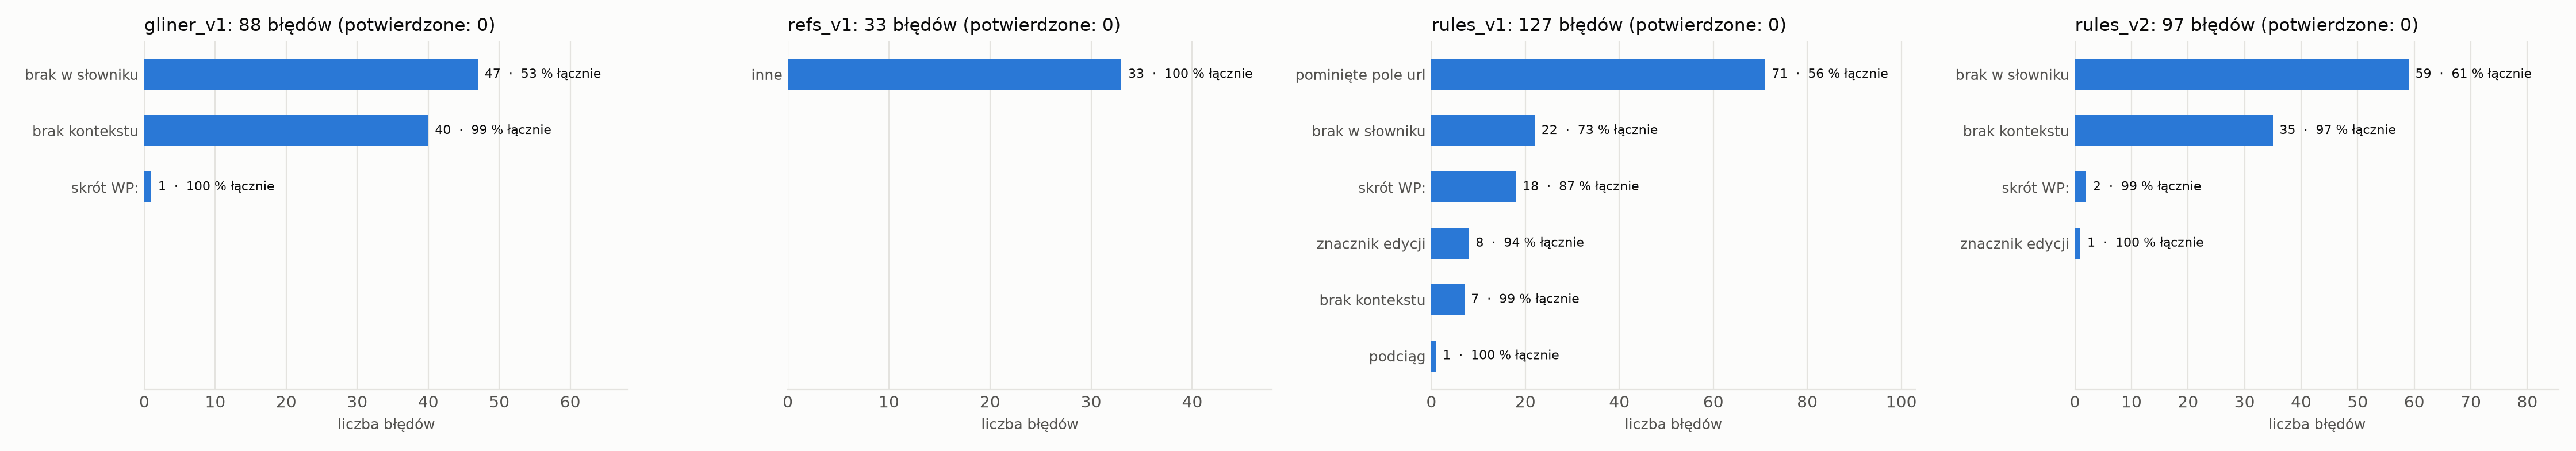
\includegraphics[width=\linewidth]{dev_pareto.png}
\caption{Błędy instrumentów na \kod{dev} według przyczyny (proponowanej, jeszcze niepotwierdzonej), z udziałem skumulowanym.}
\label{fig:pareto}
\end{figure}

\begin{table}[htbp]
\centering
\caption{Liczba błędów na \kod{dev} i najczęstsze przyczyny.}
\label{tab:bledy}
\tabela{errors}
\end{table}

Ponad połowa błędów v1 to pominięty link posta, a drugą grupą są skróty \kod{WP:} i znaczniki edycji. W regułach v2 te przyczyny prawie znikają. U obu nowszych instrumentów dominują braki w słowniku i brak kontekstu, czyli źródła nienazwane wprost albo nazwy użyte nie w funkcji źródła (R2). Wszystkie błędy I4 to rozbieżność konstruktu: zmiana przypisów bez deklaracji w opisie zmiany albo deklaracja bez zmiany.

\textbf{Błąd różnicowy.} Jeśli instrument myli się inaczej w różnych latach lub grupach, porównania w czasie są obciążone. Tabela~\ref{tab:roznicowy} podaje wartości $p$ testu permutacyjnego dla odsetka fałszywych trafień (FP, wśród jednostek bez powołania w gold) i pominięć (FN, wśród jednostek z powołaniem). Porównujemy połówki okresu badania (Reddit 2005--2012 i 2013--2020, Wikipedia 2020--2022 i 2023--2026) oraz subreddity i strony.
\begin{itemize}
  \item Między połówkami okresu żaden instrument nie ma istotnie różnych błędów.
  \item Między subredditami GLiNER różni się odsetkiem fałszywych trafień ($p = 0{,}006$), ale zbiór testowy ma tylko kilkanaście postów bez powołania.
\end{itemize}
Przy tej liczbie jednostek test pozwala raczej „nie wykluczyć różnic” niż je wykluczyć.

\begin{table}[htbp]
\centering
\caption{Błąd różnicowy dla \kod{cites\_source} na zbiorze testowym: wartości $p$ testu permutacyjnego różnic w liczbie błędów między połówkami okresu i między subredditami lub stronami.}
\label{tab:roznicowy}
\tabela{differential}
\uwaga{„--”: brak błędów danego rodzaju, więc nie ma czego porównywać.}
\end{table}

\section{Porównanie instrumentów i wybór}
\label{sec:porownanie}

Instrumenty porównujemy trzema miarami: $\kappa$ instrumentów względem gold na tle $\kappa$ annotatorów (tabela~\ref{tab:kappa}), dokładny test McNemara \cite{mcnemar1947} dla par instrumentów (tabela~\ref{tab:mcnemar}) i $\tau$ Kendalla \cite{kendall1938} między rankingiem kategorii według instrumentu a według gold (tabela~\ref{tab:rankingi}). Wyniki:
\begin{itemize}
  \item \textbf{GLiNER a pozostałe instrumenty:} GLiNER wypada istotnie lepiej od zero-shot i od v1 na obu platformach.
  \item \textbf{$\kappa$ annotatorów:} wynosi 0 przy 91\% zgodności (paradoks rozpowszechnienia), więc nie nadaje się na próg.
  \item \textbf{Ranking kategorii:} żaden instrument nie wskazuje tej samej najczęstszej kategorii co gold. Na Reddicie gold ma media informacyjne, a GLiNER media społecznościowe. Wniosek z EDA o tym, na co powołują się użytkownicy, zależy więc od instrumentu.
\end{itemize}

\begin{table}[htbp]
\centering
\caption{$\kappa$ Cohena instrumentów względem gold (zbiór testowy) i annotatorów między sobą (pilotaż), z odsetkiem zgodności.}
\label{tab:kappa}
\tabela{kappa}
\end{table}

\begin{table}[htbp]
\centering
\caption{Dokładny test McNemara dla \kod{cites\_source} na zbiorze testowym: liczba jednostek, w których trafnie klasyfikuje tylko jeden instrument z pary.}
\label{tab:mcnemar}
\tabela{mcnemar}
\end{table}

\begin{table}[htbp]
\centering
\caption{Zgodność rankingu kategorii (ważone udziały na zbiorze testowym) z rankingiem według gold: $\tau_b$ Kendalla.}
\label{tab:rankingi}
\tabela{rankings}
\end{table}

\textbf{Wybór instrumentu do bloku 4.} Reguła wyboru została zapisana z góry: wybieramy najprostszy instrument, którego zgodność z gold nie jest wyraźnie niższa niż zgodność ludzi, a przy remisie tańszy i deterministyczny. Według niej:
\begin{itemize}
  \item na Reddicie używamy GLiNER-a dla \kod{cites\_source} oraz kategorii \kod{media} i \kod{social\_blog}, a reguły v2 są kandydatem do sprawdzenia na teście;
  \item na Wikipedii typów źródeł nie liczymy automatycznie;
  \item dla \kod{edit\_about\_sources} rozstrzygnie test reguł v2 i I4.
\end{itemize}

\section{Weryfikacja hipotez}
\label{sec:hipotezy}

Preregistracja (commit \kod{440b5fb}) określa wskaźniki, model i warunki trafności. Trend mierzymy ważoną regresją logistyczną z efektami stałymi subredditu (H1) albo strony (H2) i błędami grupowanymi po wylosowanym dniu albo rewizji. Testujemy jednostronnie, przy $\alpha = 0{,}05$.

Przebieg potwierdzający wykonaliśmy z trzema zapisanymi odstępstwami:
\begin{itemize}
  \item przegląd domen wykonał tylko asystent AI;
  \item nie wykonano audytu kategorii;
  \item test H1-A czeka na etykiety stanowiska.
\end{itemize}
Rysunek~\ref{fig:udzialy} pokazuje roczne udziały.

\begin{figure}[htbp]
\centering
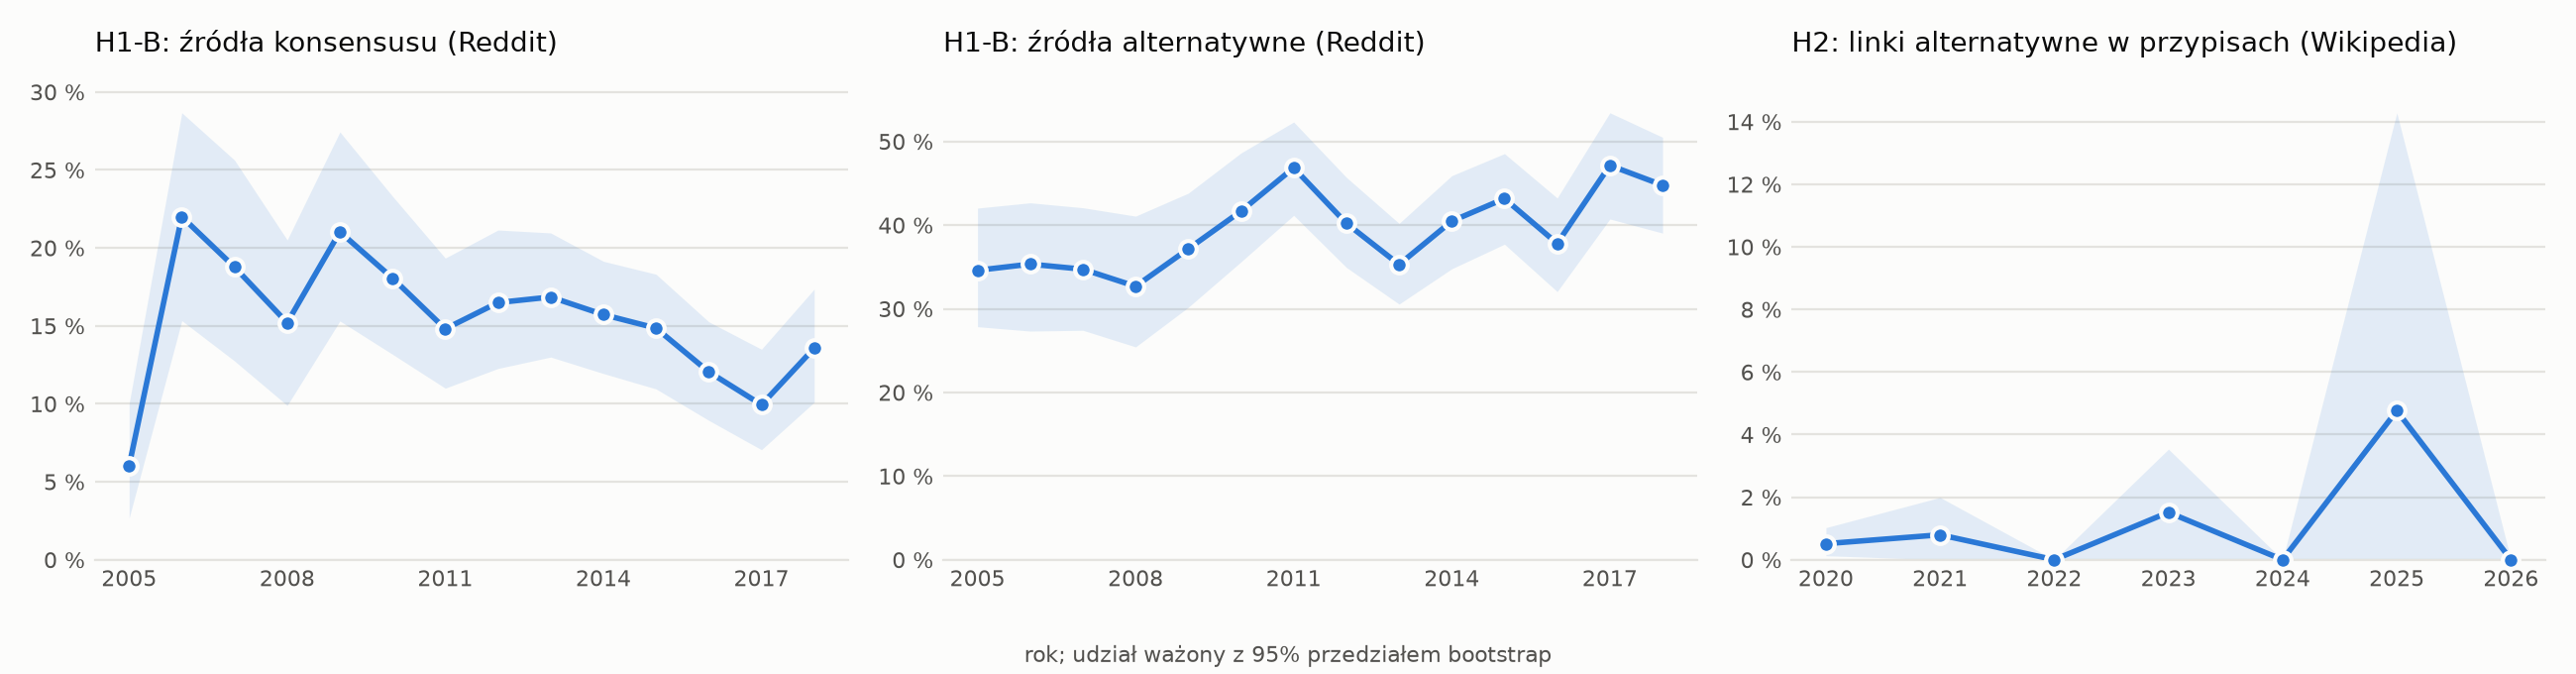
\includegraphics[width=\linewidth]{yearly_shares.png}
\caption{Roczne ważone udziały wskaźników H1-B (wśród postów z powołaniem, \kod{gliner\_v1}) i H2 (wśród linków dodanych do przypisów), z 95\% przedziałami bootstrap.}
\label{fig:udzialy}
\end{figure}

\subsection{H1: zaufanie do konsensusu naukowego}

Test główny H1-A (udział postów podważających konsensus) wymaga ludzkich etykiet stanowiska i nastrojenia instrumentu \kod{stance\_v1}, więc jeszcze się nie odbył. Wskaźniki poboczne H1-B liczymy na próbie 6240 postów z czterech subredditów:
\begin{itemize}
  \item \textbf{Surowe udziały} zmieniają się w kierunku hipotezy: źródła konsensusu spadają z około 22\% w 2006~r. do 10--14\% w latach 2016--2018, a źródła alternatywne rosną z około 35\% do 45--47\%.
  \item \textbf{Trend w modelu} znika po uwzględnieniu subredditu, także osobno w r/science i w r/conspiracy (tabela~\ref{tab:h1b}). Zmiana w danych łącznych wynika ze zmiany składu, czyli rosnącego udziału r/conspiracy.
\end{itemize}
Wskaźnik konsensusu raportujemy tylko opisowo, bo nie przeszedł audytu. Sposób liczenia audytu doprecyzowaliśmy przed jego kodowaniem (poprawka z 25.10.2026): wagi $1/\pi$, połączenie z gold i korekta Rogana--Gladena \cite{rogan1978}.

\begin{table}[htbp]
\centering
\caption{H1-B: trend wskaźników źródeł (iloraz szans na rok, efekty stałe subredditu). Wartość $p$ jednostronna w kierunku hipotezy.}
\label{tab:h1b}
\szeroka{h1b}
\end{table}

\subsection{H2: źródła alternatywne w Wikipedii}

\textbf{Test z preregistracji.} W latach 2020--2026 do przypisów ośmiu stron dodano 1341 linków, z czego 10 z domen alternatywnych. Test główny daje OR 1,47 na rok, $p = 0{,}006$ (tabela~\ref{tab:h2}), więc formalnie spełnia kryterium. Analizy wrażliwości i test permutacyjny nie są jednak istotne.

\textbf{Sprawdzenie pomiaru (eksploracyjne).} Odporność modelu sprawdziliśmy logitem Firtha \cite{firth1993} i modelem Poissona. Ważniejszy okazał się jednak odczyt samych linków (tabela~\ref{tab:h2odpornosc}):
\begin{itemize}
  \item 8 z 10 linków „alternatywnych” to oficjalne wpisy WHO (Periscope, jeden link dodany 6 razy przy rewertach) i Głównego Inspektoratu Sanitarnego (Twitter);
  \item po przypisaniu ich do instytucji zostają 2 linki w siedmiu latach, a test dokładny daje $p = 0{,}21$.
\end{itemize}
Formalne potwierdzenie H2 jest więc artefaktem klasyfikacji po domenie i wielokrotnego liczenia przywracanych linków. Dane nie wspierają H2. Przyszły test powinien klasyfikować źródło według właściciela konta, liczyć tylko pierwsze dodanie linku i mieć nową preregistrację.

\begin{table}[htbp]
\centering
\caption{H2: test z preregistracji i analizy wrażliwości (iloraz szans na rok, efekty stałe strony).}
\label{tab:h2}
\tabela{h2}
\end{table}

\begin{table}[htbp]
\centering
\caption{H2: analizy odporności i sprawdzenie pomiaru (eksploracyjne, spoza preregistracji).}
\label{tab:h2odpornosc}
\szeroka{h2_robustness}
\end{table}

\section{Ograniczenia}

\begin{itemize}
  \item Zgodność annotatorów w pilotażu jest niska. Gold jest podzielony między osoby i nie został jeszcze podwójnie zakodowany ani uzgodniony przez arbitra.
  \item Część gold pochodzi z etykiet wstępnych AI zatwierdzonych przez człowieka, co może sprzyjać instrumentom AI.
  \item Na Wikipedii jest mało powołań (20 w zbiorze testowym), więc przedziały są szerokie, a kategorie rzadkie nieocenialne.
  \item Reguły v2 i I4 nie przeszły jeszcze testu; ich wyniki na \kod{dev} są optymistyczne.
  \item Przyczyny błędów są proponowane przez heurystykę i czekają na potwierdzenie.
  \item Osiem stron Wikipedii wybranych tematycznie nie reprezentuje całej Wikipedii. Rok 2026 jest niepełny.
  \item Klasyfikacja po domenie nie odróżnia konta instytucji od blogera ani „eksperta niezależnego” na zwykłej stronie.
\end{itemize}

\section{Reprodukowalność i użycie AI}

\textbf{Reprodukowalność.} Kod, manifest próby, etykiety bez tekstu i wszystkie wyniki są w repozytorium. Teksty jednostek są w \kod{data\_samples/}, a arkusze z tekstem poza gitem. Każdy krok ma polecenie \kod{make}, a kolejne kroki opisuje \kod{docs/plan\_walidacji.md}. Zbiór testowy uruchamia się raz na instrument i tylko na zacommitowanym kodzie. Test potwierdzający hipotez odmawia uruchomienia, gdy pliki preregistracji nie są zacommitowane.

\textbf{Użycie AI.} Przy pracy korzystaliśmy z asystenta AI (Claude Code). Pisał kod i testy, przygotował etykiety wstępne w arkuszach JP (przejrzane i zatwierdzone przez JP), sklasyfikował listę domen dla H2 (przegląd przez człowieka jest odstępstwem zapisanym w preregistracji), zaproponował przyczyny błędów (do potwierdzenia) i przygotował projekt tego raportu. Instrumenty AI w badaniu (zero-shot, GLiNER) to lokalne modele otwarte, niezależne od asystenta.

\begin{thebibliography}{99}
\bibitem{cohen1960} J.~Cohen. A coefficient of agreement for nominal scales. \textit{Educational and Psychological Measurement}, 20(1):37--46, 1960.
\bibitem{feinstein1990} A.~R. Feinstein, D.~V. Cicchetti. High agreement but low kappa: I.~The problems of two paradoxes. \textit{Journal of Clinical Epidemiology}, 43(6):543--549, 1990.
\bibitem{firth1993} D.~Firth. Bias reduction of maximum likelihood estimates. \textit{Biometrika}, 80(1):27--38, 1993.
\bibitem{kendall1938} M.~G. Kendall. A new measure of rank correlation. \textit{Biometrika}, 30(1/2):81--93, 1938.
\bibitem{krippendorff2004} K.~Krippendorff. \textit{Content Analysis: An Introduction to Its Methodology}. Wyd.~2. Sage, 2004.
\bibitem{laurer2024} M.~Laurer, W.~van Atteveldt, A.~Casas, K.~Welbers. Less annotating, more classifying: Addressing the data scarcity issue of supervised machine learning with deep transfer learning and BERT-NLI. \textit{Political Analysis}, 32(1):84--100, 2024.
\bibitem{mcnemar1947} Q.~McNemar. Note on the sampling error of the difference between correlated proportions or percentages. \textit{Psychometrika}, 12(2):153--157, 1947.
\bibitem{passonneau2006} R.~Passonneau. Measuring agreement on set-valued items (MASI) for semantic and pragmatic annotation. W: \textit{Proceedings of LREC 2006}, 2006.
\bibitem{rogan1978} W.~J. Rogan, B.~Gladen. Estimating prevalence from the results of a screening test. \textit{American Journal of Epidemiology}, 107(1):71--76, 1978.
\bibitem{zaratiana2024} U.~Zaratiana, N.~Tomeh, P.~Holat, T.~Charnois. GLiNER: Generalist model for named entity recognition using bidirectional transformer. W: \textit{Proceedings of NAACL 2024}, 2024.
\end{thebibliography}

\end{document}
